
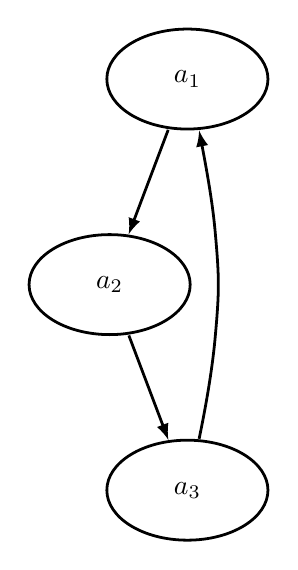
\begin{tikzpicture}[>=latex,line join=bevel,]
  \pgfsetlinewidth{1bp}
%%
\pgfsetcolor{black}
  % Edge: a_2 -> a_3
  \draw [->] (35.921bp,74.708bp) .. controls (39.143bp,66.195bp) and (43.042bp,55.888bp)  .. (50.158bp,37.082bp);
  % Edge: a_3 -> a_1
  \draw [->] (61.215bp,37.471bp) .. controls (63.423bp,48.092bp) and (65.893bp,61.724bp)  .. (67bp,74bp) .. controls (68.517bp,90.821bp) and (68.517bp,95.179bp)  .. (67bp,112bp) .. controls (66.213bp,120.73bp) and (64.737bp,130.14bp)  .. (61.215bp,148.53bp);
  % Edge: a_1 -> a_2
  \draw [->] (50.079bp,148.71bp) .. controls (46.857bp,140.19bp) and (42.958bp,129.89bp)  .. (35.842bp,111.08bp);
  % Node: a_3
\begin{scope}
  \definecolor{strokecol}{rgb}{0.0,0.0,0.0};
  \pgfsetstrokecolor{strokecol}
  \draw (57bp,19bp) ellipse (29bp and 18bp);
  \draw (57bp,19bp) node {$a_3$};
\end{scope}
  % Node: a_2
\begin{scope}
  \definecolor{strokecol}{rgb}{0.0,0.0,0.0};
  \pgfsetstrokecolor{strokecol}
  \draw (29bp,93bp) ellipse (29bp and 18bp);
  \draw (29bp,93bp) node {$a_2$};
\end{scope}
  % Node: a_1
\begin{scope}
  \definecolor{strokecol}{rgb}{0.0,0.0,0.0};
  \pgfsetstrokecolor{strokecol}
  \draw (57bp,167bp) ellipse (29bp and 18bp);
  \draw (57bp,167bp) node {$a_1$};
\end{scope}
%
\end{tikzpicture}

